\documentclass[12pt, a4paper]{report}
\usepackage[top=1cm, left=0.8cm, right=0.8cm]{geometry}

\usepackage[utf8]{inputenc}
\usepackage[russian]{babel}

\usepackage{array}
\newcolumntype{M}[1]{>{\centering\arraybackslash}m{#1}}

\usepackage{hyperref}
\hypersetup{
	colorlinks,
	citecolor=black,
	filecolor=black,
	linkcolor=black,
	urlcolor=black
}

\usepackage{sectsty}
\allsectionsfont{\centering}

\usepackage{indentfirst}
\setlength\parindent{24pt}
 
\usepackage{listings}
\usepackage{xcolor}
\definecolor{codegreen}{rgb}{0,0.6,0}
\definecolor{codegray}{rgb}{0.5,0.5,0.5}
\definecolor{codepurple}{rgb}{0.58,0,0.82}
\definecolor{backcolour}{rgb}{0.95,0.95,0.92}
\lstdefinestyle{mystyle}{
    backgroundcolor=\color{backcolour},
    commentstyle=\color{codegreen},
    keywordstyle=\color{magenta},
    numberstyle=\normalsize\color{codegray},
    stringstyle=\color{codepurple},
    basicstyle=\ttfamily\footnotesize,
    breakatwhitespace=false,
    breaklines=true,
    captionpos=b,
    keepspaces=true,
    numbers=left,
    numbersep=5pt,
    showspaces=false,
    showstringspaces=false,
    showtabs=false,
    tabsize=2
}

\usepackage{graphicx}
\graphicspath{{assets/}}

\begin{document}
	\begin{titlepage}
		\begin{center}
			\large \textbf{Министерство науки и высшего образования Российской Федерации} \\
			\large \textbf{Федеральное государственное бюджетное образовательное учреждение высшего образования} \\
			\large \textbf{«Российский химико-технологический университет имени Д.И. Менделеева»} \\

			\vspace*{4cm}
			\LARGE \textbf{ОТЧЕТ ПО ЛАБОРАТОРНОЙ РАБОТЕ №6}

			\vspace*{4cm}
			\begin{flushright}
				\Large
				\begin{tabular}{>{\raggedleft\arraybackslash}p{8.85cm} p{10.8cm}}
					Выполнил студент группы КС-36: & Золотухин Андрей Александрович \\
					Ссылка на репозиторий: & https://github.com/ \\ 
					& CorgiPuppy/ \\
					& info-sys-admin-labs \\
					Принял: & Митричев Иван Игоревич \\
					Дата сдачи: & 09.04.2025 \\
				\end{tabular}

			\end{flushright}

			\vspace*{6cm}
			\Large \textbf{Москва \\ 2025}
		\end{center}
	\end{titlepage}
	
	\tableofcontents	
	\thispagestyle{empty}
	\newpage

	\pagenumbering{arabic}
	
	\section*{Описание и выполнение задачи}
	\addcontentsline{toc}{section}{Описание и выполнение задачи}	
	\large
	Задания 1-19 выполняются в терминале (bash) со скриншотами. \par

	\subsection*{Задание 1}
	\addcontentsline{toc}{subsection}{Задание 1}
	\begin{enumerate}
		\item Создайте файл \textit{example.txt} в домашней директории;
		\item Установите права доступа для файла в формате \underline{644} (владелец может читать и записывать, группа и остальные могут только читать).
	\end{enumerate}
	\lstset{style=mystyle}
	\lstinputlisting[language=Bash]{src/task1/main.sh}
	\begin{center}
		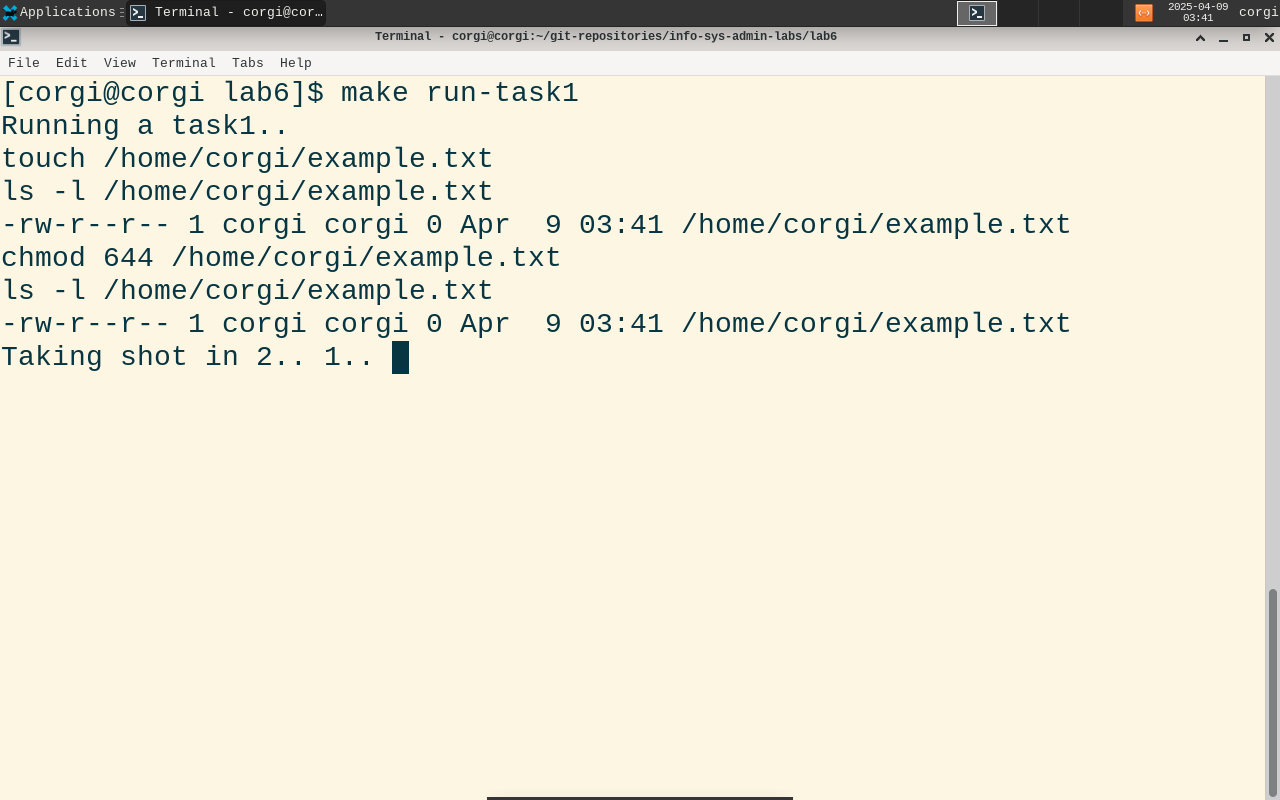
\includegraphics[width=500pt]{task1.png}
	\end{center}

	\subsection*{Задание 2}
	\addcontentsline{toc}{subsection}{Задание 2}
	\begin{enumerate}
		\item Измените права доступа для файла \textit{example.txt} на \underline{600} (только владелец может читать и записывать);
		\item Проверьте права доступа с помощью команды \textit{ls -l}.
	\end{enumerate}
	\lstset{style=mystyle}
	\lstinputlisting[language=Bash]{src/task2/main.sh}
	\begin{center}
		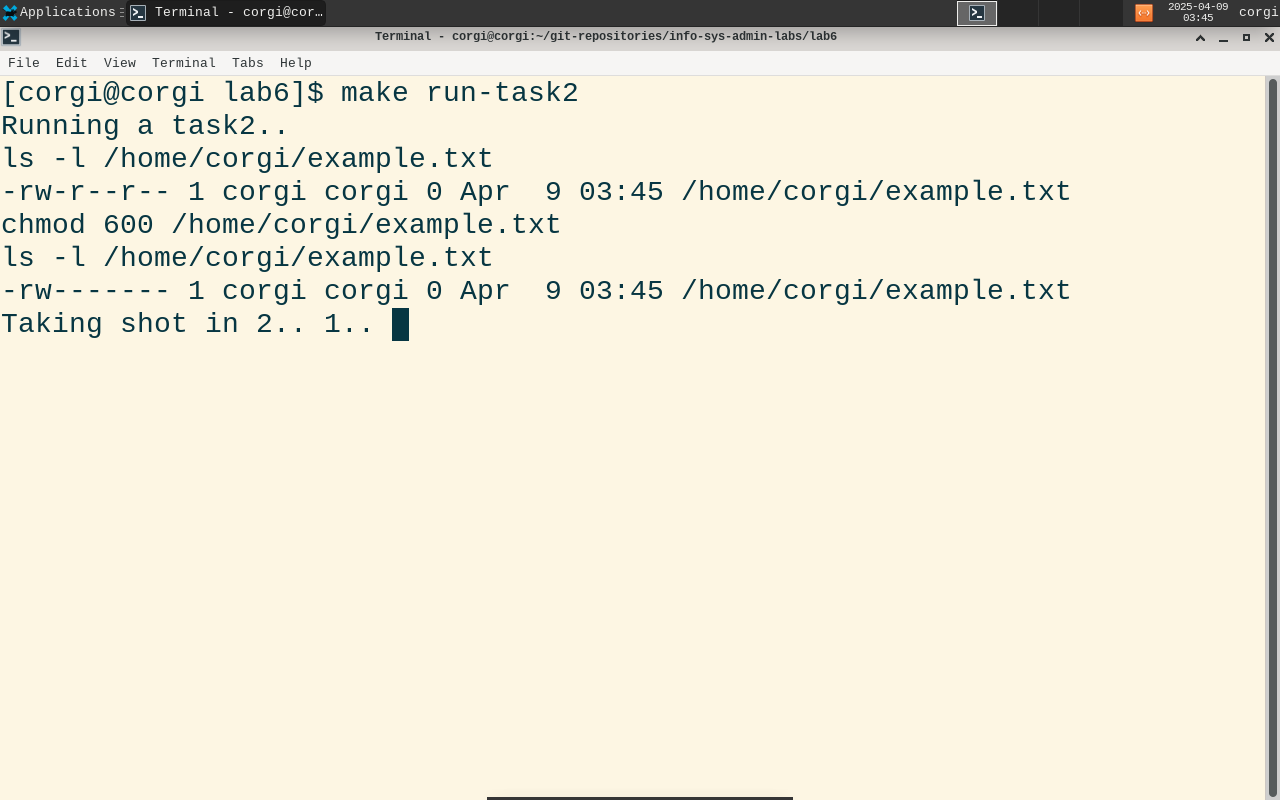
\includegraphics[width=500pt]{task2.png}
	\end{center}

	\subsection*{Задание 3}
	\addcontentsline{toc}{subsection}{Задание 3}
	\begin{enumerate}
		\item Создайте директорию \textit{mydir};
		\item Установите права доступа для директории в формате \underline{755} (владелец может читать, записывать и выполнять, группа и остальные могут только читать и выполнять;
		\item Создайте непустой файл \textit{mydir/file2.txt}, права по умолчанию;
		\item Попытайтесь изменить файл на \textit{file2.txt}. Объясните результат;
		\item Смените права на \textit{file2.txt} на \underline{400}. Попытайтесь изменить файл \textit{file2.txt}. Объясните результат;
		\item Попытайтесь удалить \textit{file2.txt}. Объясните результат.
	\end{enumerate}
	\lstset{style=mystyle}
	\lstinputlisting[language=Bash]{src/task3/main.sh}
	\begin{center}
		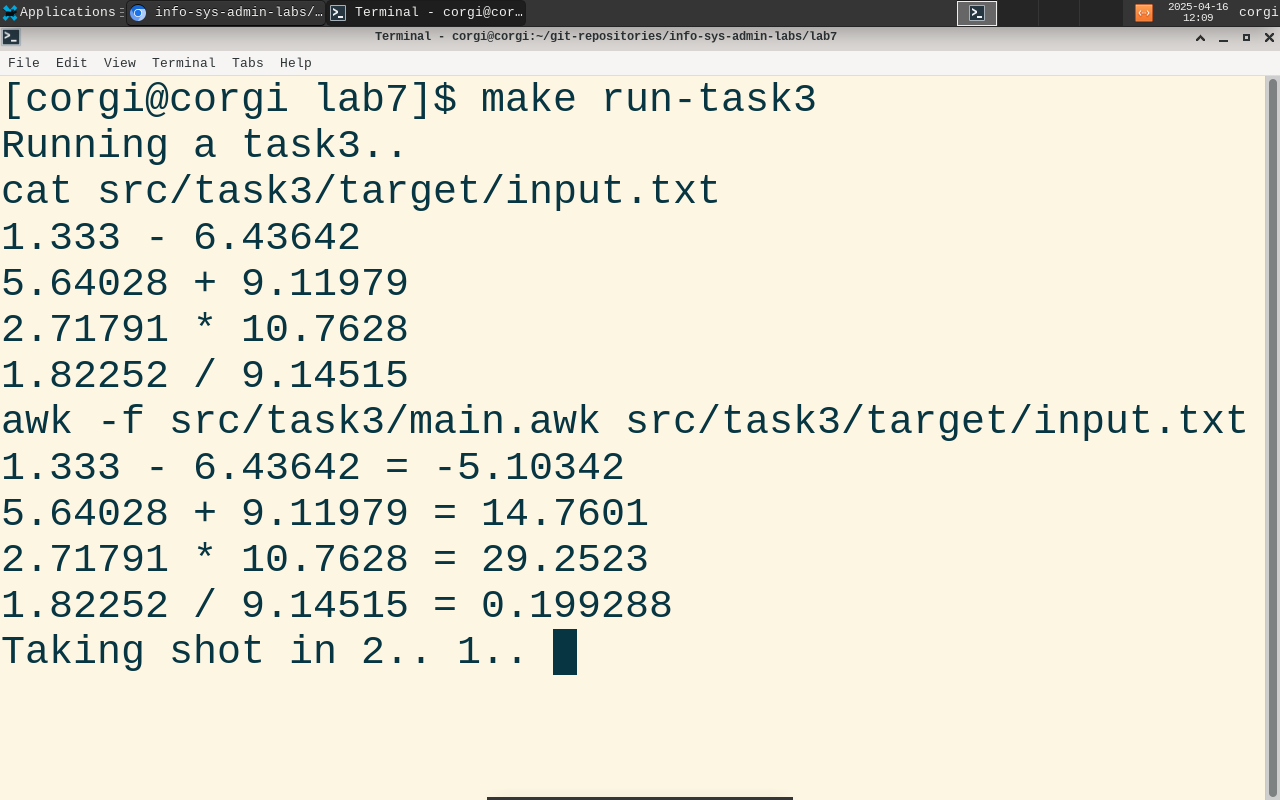
\includegraphics[width=500pt]{task3.png}
	\end{center}

	\subsection*{Задание 4}
	\addcontentsline{toc}{subsection}{Задание 4}
	\begin{enumerate}
		\item Создайте файл \textit{script.sh} в \textit{mydir};
		\item Установите права доступа для файла в буквенном формате так, чтобы владелец мог читать, записывать и выполнять, а группа и остальные пользователи не имели прав (то есть \underline{rwx------}).
	\end{enumerate}
	\lstset{style=mystyle}
	\lstinputlisting[language=Bash]{src/task4/main.sh}
	\begin{center}
		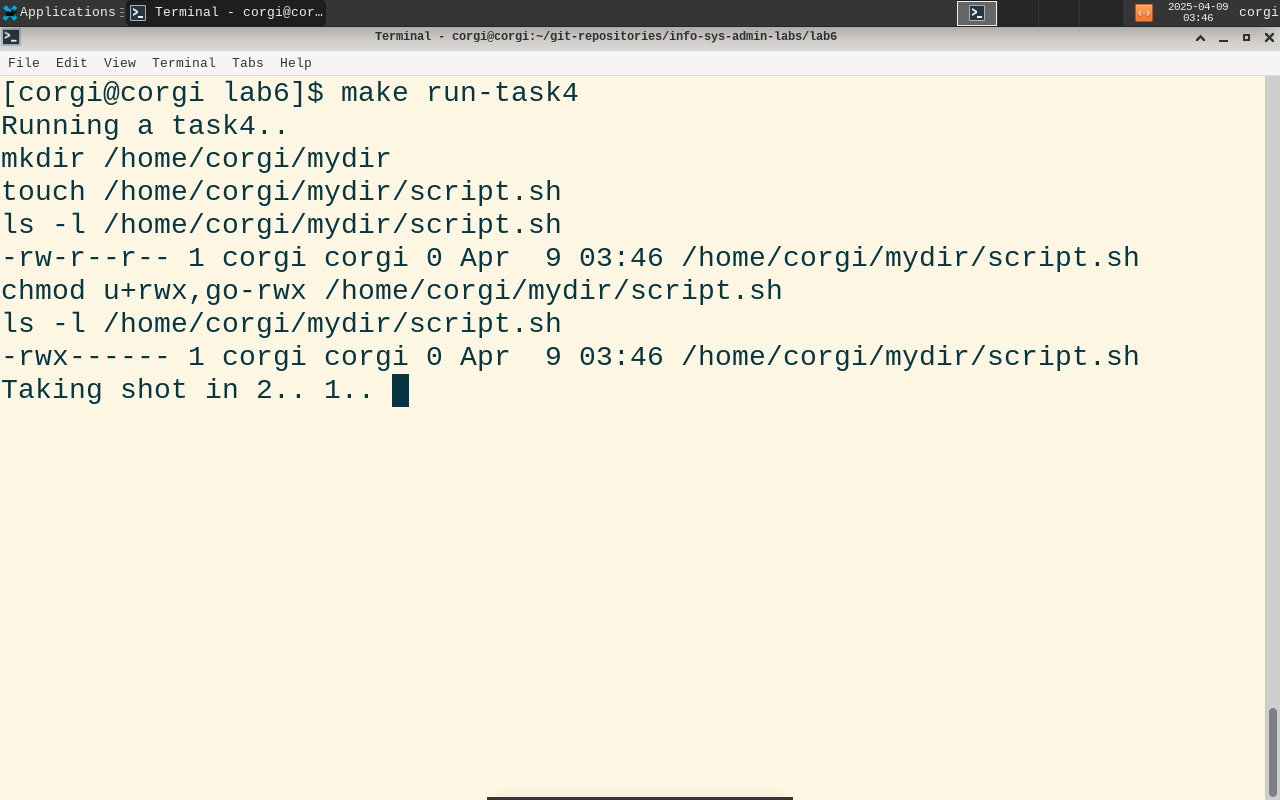
\includegraphics[width=500pt]{task4.png}
	\end{center}

	\subsection*{Задание 5}
	\addcontentsline{toc}{subsection}{Задание 5}
	\begin{enumerate}
		\item Создайте поддиректорию \textit{subdir} в \textit{mydir};
		\item Установите права доступа для \textit{subdir} и всех файлов в ней так, чтобы только владелец мог читать и записывать (то есть \underline{700}).
	\end{enumerate}
	\lstset{style=mystyle}
	\lstinputlisting[language=Bash]{src/task5/main.sh}
	\begin{center}
		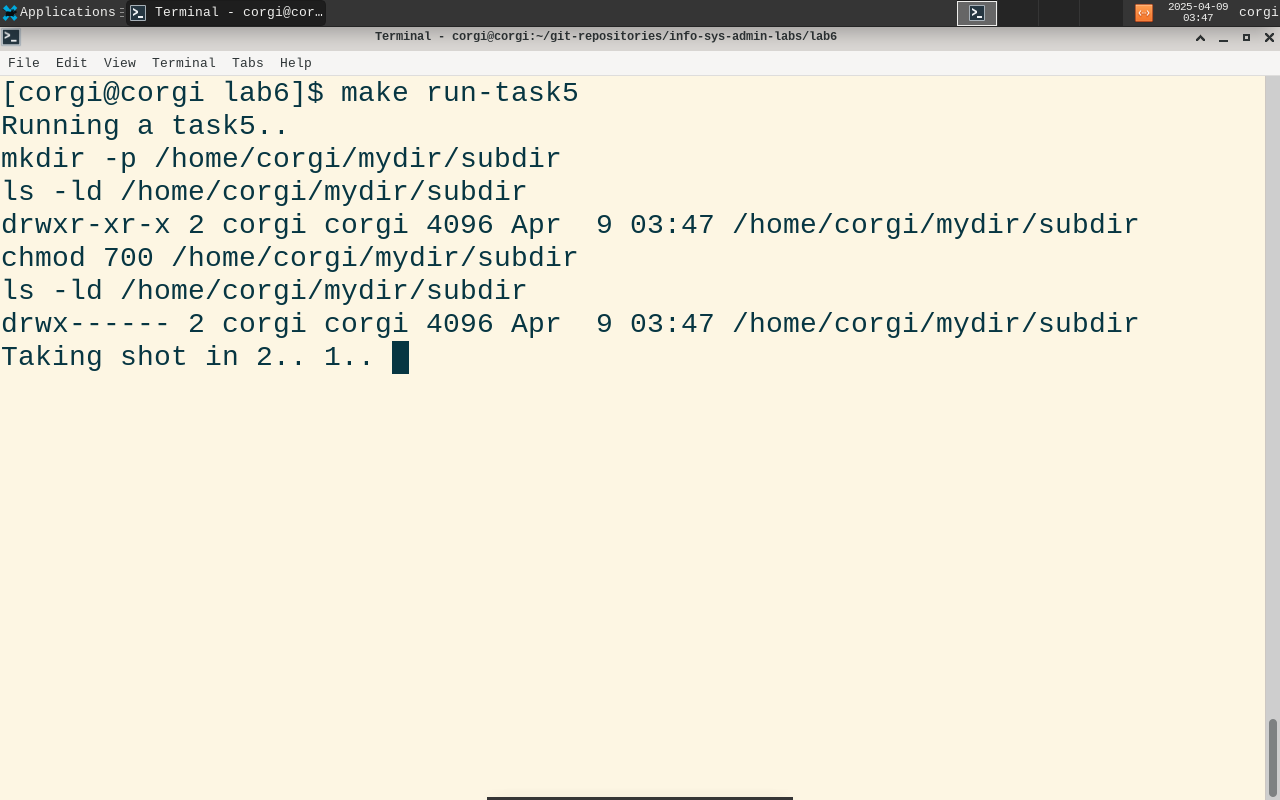
\includegraphics[width=500pt]{task5.png}
	\end{center}

	\subsection*{Задание 6}
	\addcontentsline{toc}{subsection}{Задание 6}
	\begin{enumerate}
		\item Создайте непустой файл \textit{mydir/file3.txt}, права по умолчанию;
		\item Измените права доступа для директории \textit{mydir} на \underline{600} (только владелец может читать, записывать);
		\item Проверьте права доступа с помощью команды \textit{ls -ld};
		\item Попытайтесь удалить \textit{file3.txt}. Объясните результат;
		\item Попытайтесь изменить \textit{file3.txt}. Объясните результат.
	\end{enumerate}
	\lstset{style=mystyle}
	\lstinputlisting[language=Bash]{src/task6/main.sh}
	\begin{center}
		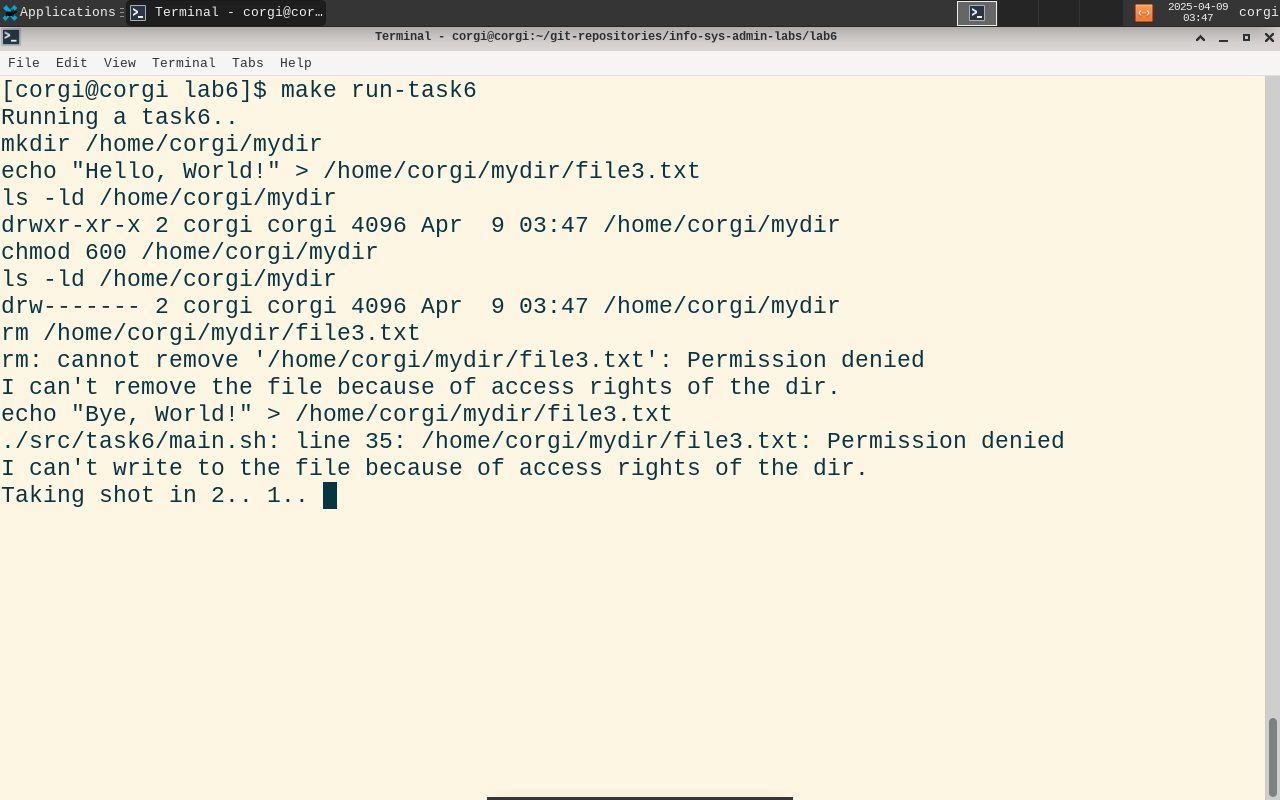
\includegraphics[width=500pt]{task6.png}
	\end{center}

	\subsection*{Задание 7}
	\addcontentsline{toc}{subsection}{Задание 6}
	На каталог \textit{d1} установлены права \underline{drwx------}. Какие права доступа минимально должны быть дополнительно установлены, чтобы \textit{user1} смог изменить файл \textit{f1} (права \textit{-r--r--r--}) в каталоге \textit{d1} (если \textit{user1} является \underline{владельцем} \underline{файла}, но \textbf{не} является \underline{владельцем} \underline{каталога})? Объясните ответ.

	\subsection*{Задание 8}
	\addcontentsline{toc}{subsection}{Задание 8}
	На каталог \textit{d1} установлены права \underline{drwx------}. Какие права доступа минимально должны быть дополнительно установлены, чтобы \textit{user1} смог изменить файл \textit{f1} (права \textit{-r--r--r--}) в каталоге \textit{d1} (если \textit{user1} \textbf{не} является \underline{владельцем} \underline{файла} и \textbf{не} является \underline{владельцем} \underline{каталога})? Объясните ответ.

	\subsection*{Задание 9}
	\addcontentsline{toc}{subsection}{Задание 9}
	На каталог \textit{d1} установлены права \underline{drwx------}. Какие права доступа минимально должны быть дополнительно установлены, чтобы \textit{user1} смог изменить файл \textit{f1} (права \textit{-r--r--r--}) в каталоге \textit{d1} (если \textit{user1} \textbf{не} является \underline{владельцем} \underline{файла}, но является \underline{владельцем} \underline{каталога})? Объясните ответ.

	\subsection*{Задание 10}
	\addcontentsline{toc}{subsection}{Задание 10}
	\begin{enumerate}
		\item Создайте новую директорию \textit{test\_dir};
		\item Установите права доступа так, чтобы только владелец мог читать, записывать и выполнять файлы в этой директории;
		\item Создайте файл \textit{file1.txt} в директории \textit{test\_dir};
		\item Установите права доступа для файла так, чтобы владелец мог читать и записывать, а группа и остальные пользователи могли только читать.
	\end{enumerate}
	\lstset{style=mystyle}
	\lstinputlisting[language=Bash]{src/task10/main.sh}
	\begin{center}
		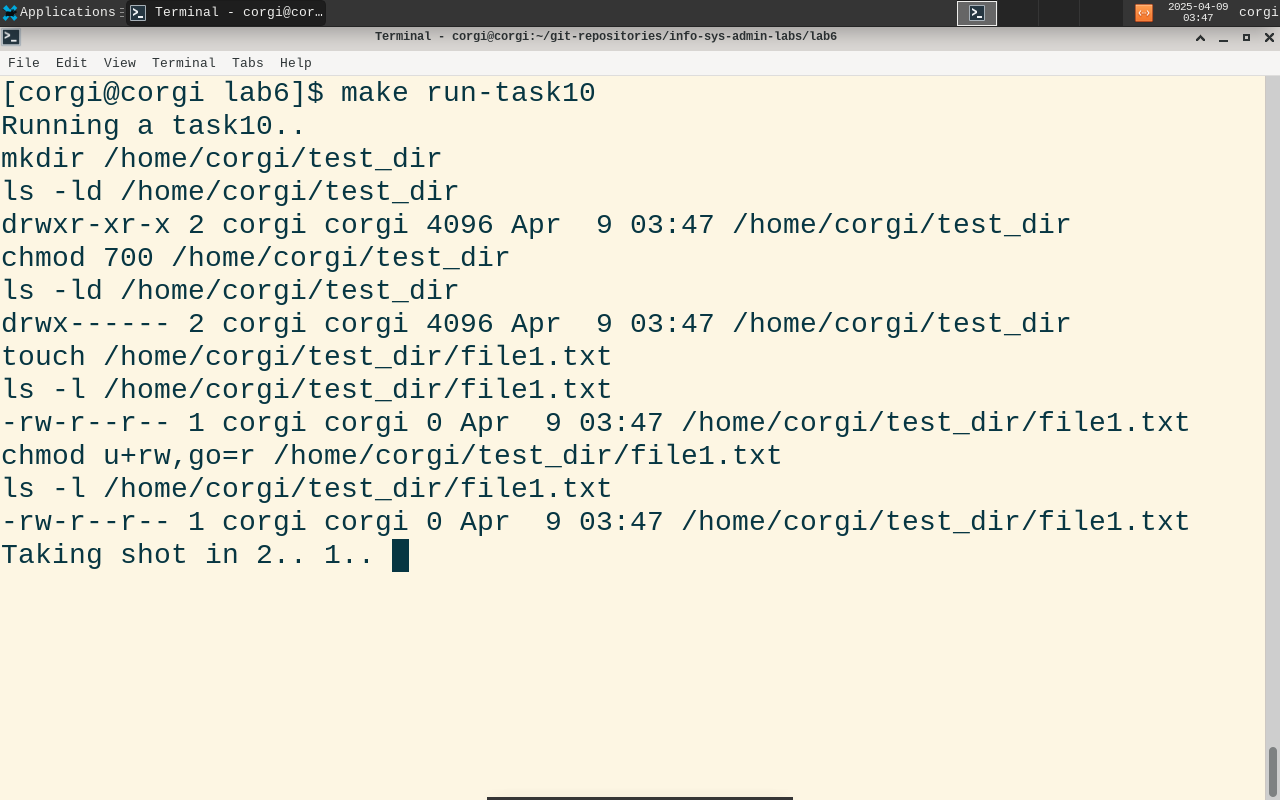
\includegraphics[width=500pt]{task10.png}
	\end{center}

	\subsection*{Задание 11}
	\addcontentsline{toc}{subsection}{Задание 11}
	\begin{enumerate}
		\item Зарегистрируйте пользователя \underline{user1}, для которого запрещён вход в сеанс, имеющего домашний каталог \textit{/home/test1};
		\item Зарегистрируйте пользователя \underline{user2}, для которого оболочкой является \textit{/bin/bash}, имеющего домашний каталог \textit{/home/user2}.
	\end{enumerate}
	\lstset{style=mystyle}
	\lstinputlisting[language=Bash]{src/task11/main.sh}
	\begin{center}
		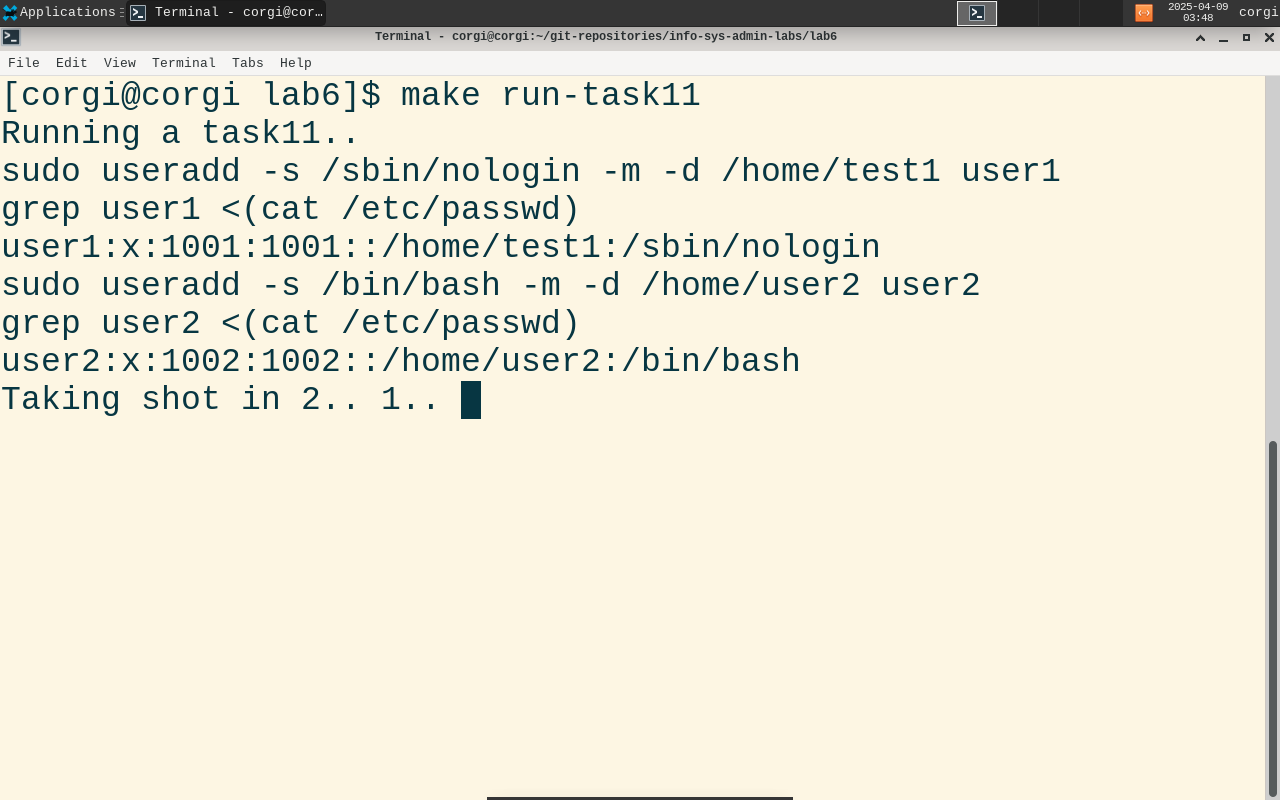
\includegraphics[width=500pt]{task11.png}
	\end{center}

	\subsection*{Задание 12}
	\addcontentsline{toc}{subsection}{Задание 12}
	\begin{enumerate}
		\item Уставновите \underline{ACL} для файла \textit{file1.txt}, чтобы пользователь \textit{user2} имел право на запись в этот файл;
		\item Проверьте, что права доступа были успешно изменены;
		\item Используйте команду \textit{getfacl} и \textit{ls -l} для вывода прав на \textit{file1.txt}.
	\end{enumerate}
	\lstset{style=mystyle}
	\lstinputlisting[language=Bash]{src/task12/main.sh}
	\begin{center}
		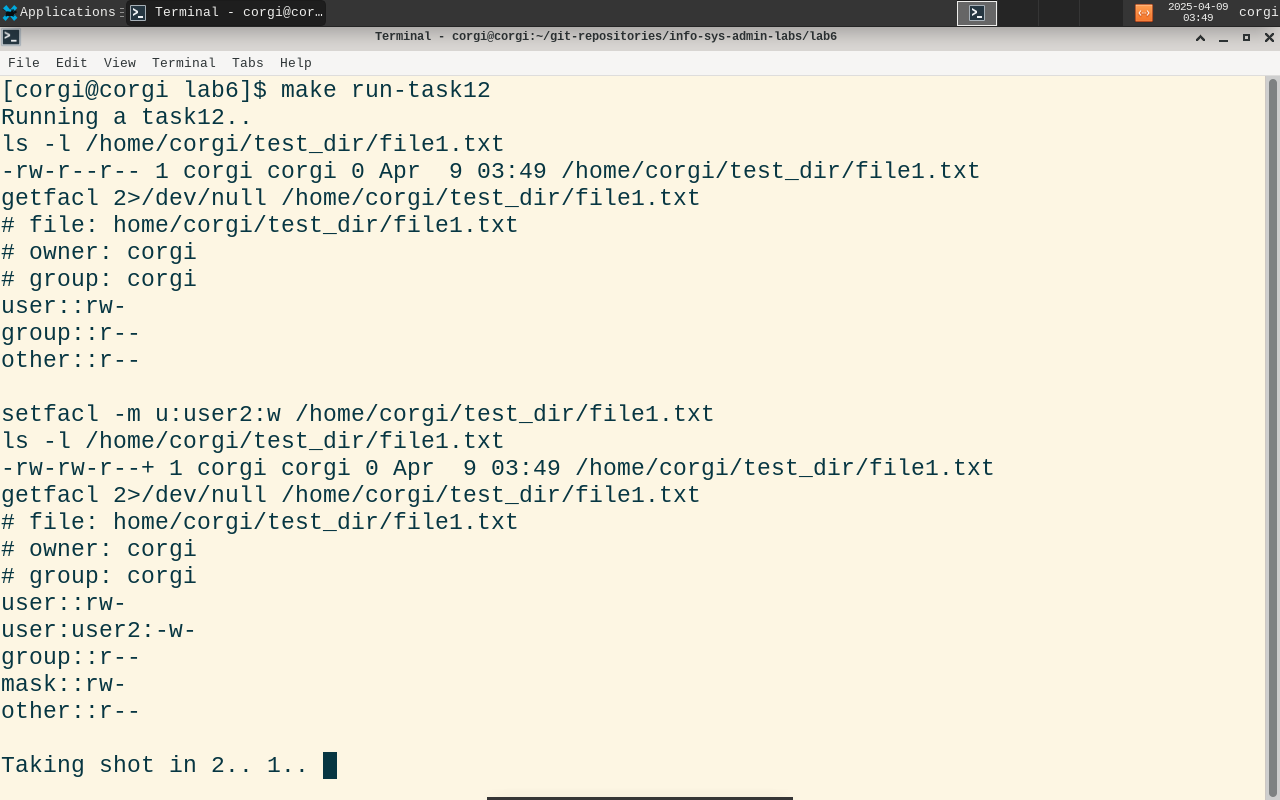
\includegraphics[width=500pt]{task12.png}
	\end{center}

	\subsection*{Задание 13}
	\addcontentsline{toc}{subsection}{Задание 13}
	\begin{enumerate}
		\item Удалите права доступа для пользователя \textit{user2} к файлу \textit{file1.txt};
		\item Проверьте, что пользователь \textit{user2} больше не имеет прав на запись.
	\end{enumerate}
	\lstset{style=mystyle}
	\lstinputlisting[language=Bash]{src/task13/main.sh}
	\begin{center}
		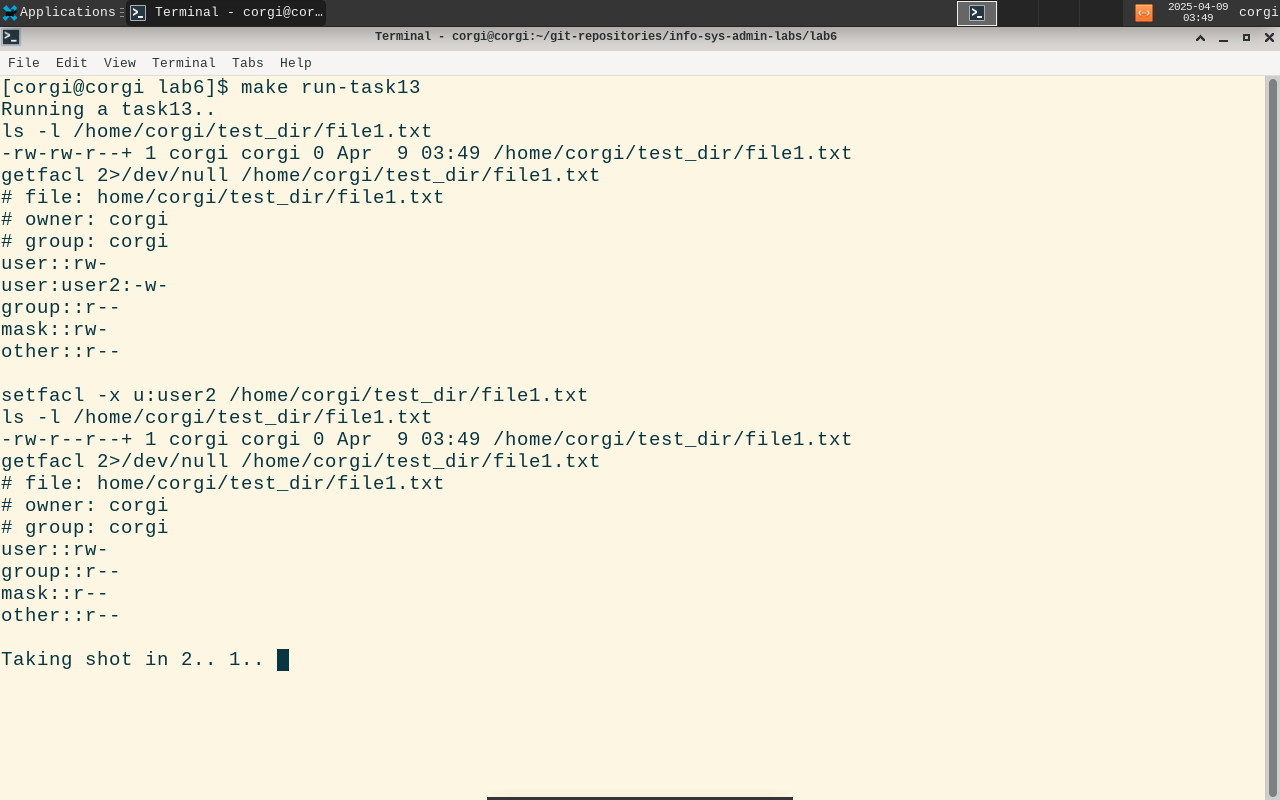
\includegraphics[width=500pt]{task13.png}
	\end{center}

	\subsection*{Задание 14}
	\addcontentsline{toc}{subsection}{Задание 14}
	\begin{enumerate}
		\item Создайте группу \textit{mygroup} и добавьте пользователей \textit{user1} и \textit{user2} в эту группу;
		\item Установите права доступа для директории \textit{test\_dir}, чтобы все члены группы \textit{mygroup} могли читать и выполнять файлы, но не могли записывать.
	\end{enumerate}
	\lstset{style=mystyle}
	\lstinputlisting[language=Bash]{src/task14/main.sh}
	\begin{center}
		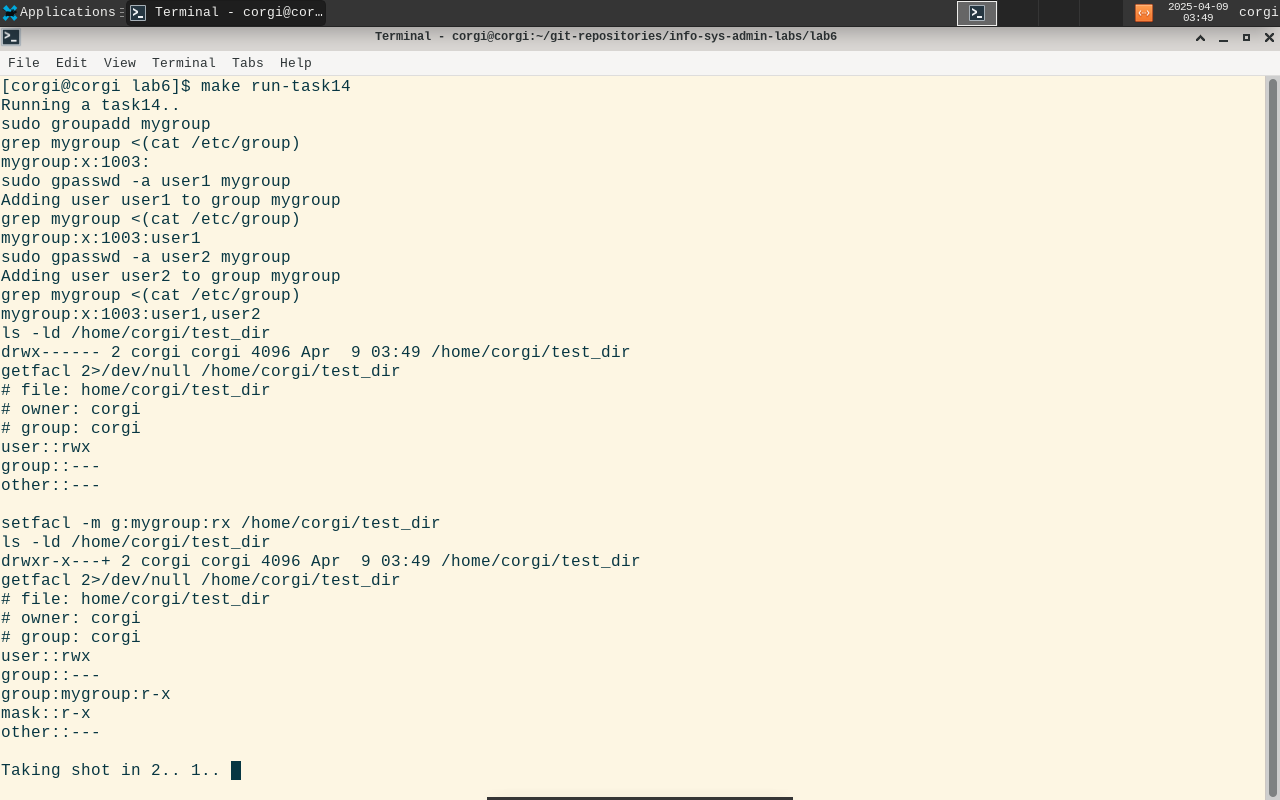
\includegraphics[width=500pt]{task14.png}
	\end{center}

	\subsection*{Задание 15}
	\addcontentsline{toc}{subsection}{Задание 15}
	\begin{enumerate}
		\item Установите умолчания \underline{ACL} для директории \textit{test\_dir}, чтобы все новые файлы, созданные в этой директории, автоматически наследовали права на чтение и запись для группы \textit{mygroup}.
	\end{enumerate}
	\lstset{style=mystyle}
	\lstinputlisting[language=Bash]{src/task15/main.sh}
	\begin{center}
		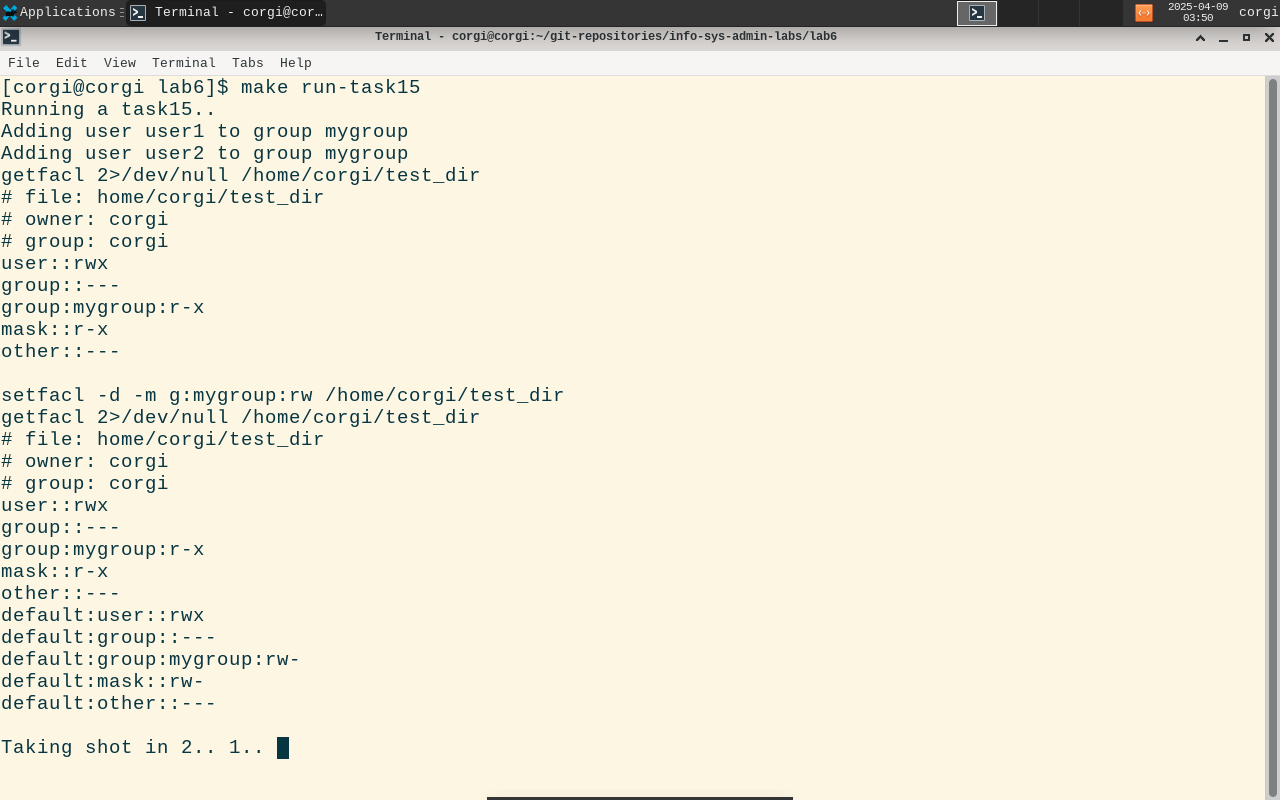
\includegraphics[width=500pt]{task15.png}
	\end{center}

	\subsection*{Задание 16}
	\addcontentsline{toc}{subsection}{Задание 16}
	\begin{enumerate}
		\item Создайте новый файл \textit{file2.txt} в директории \textit{test\_dir};
		\item Проверьте, какие права доступа установлены для этого файла, и убедитесь, что они соответствуют установленным умолчаниям.
	\end{enumerate}
	\lstset{style=mystyle}
	\lstinputlisting[language=Bash]{src/task16/main.sh}
	\begin{center}
		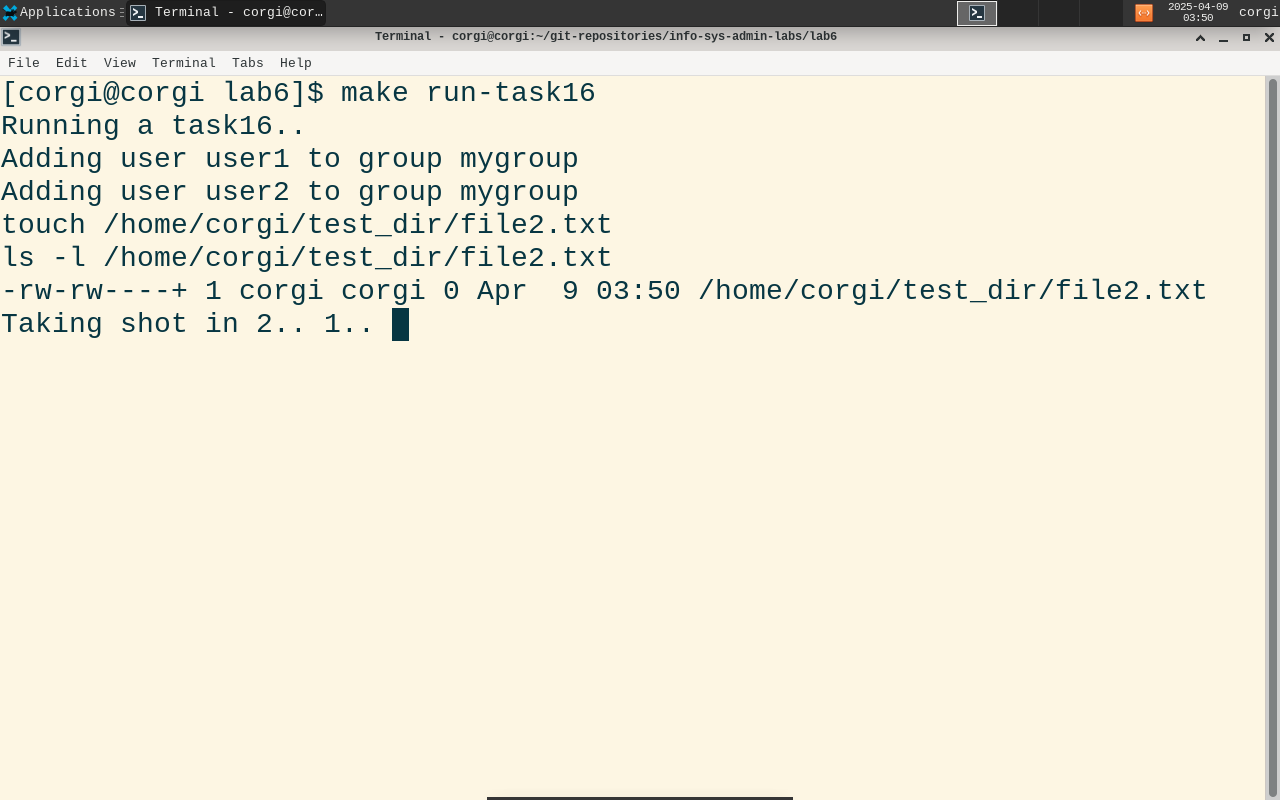
\includegraphics[width=500pt]{task16.png}
	\end{center}

	\subsection*{Задание 17}
	\addcontentsline{toc}{subsection}{Задание 17}
	\begin{enumerate}
		\item Создайте поддиректорию \textit{subdir} в \textit{test\_dir};
		\item Установите права доступа для \textit{subdir} и всех файлов в ней так, чтобы только владелец мог читать и записывать, а группа и остальные пользователи не имели прав.
	\end{enumerate}
	\lstset{style=mystyle}
	\lstinputlisting[language=Bash]{src/task17/main.sh}
	\begin{center}
		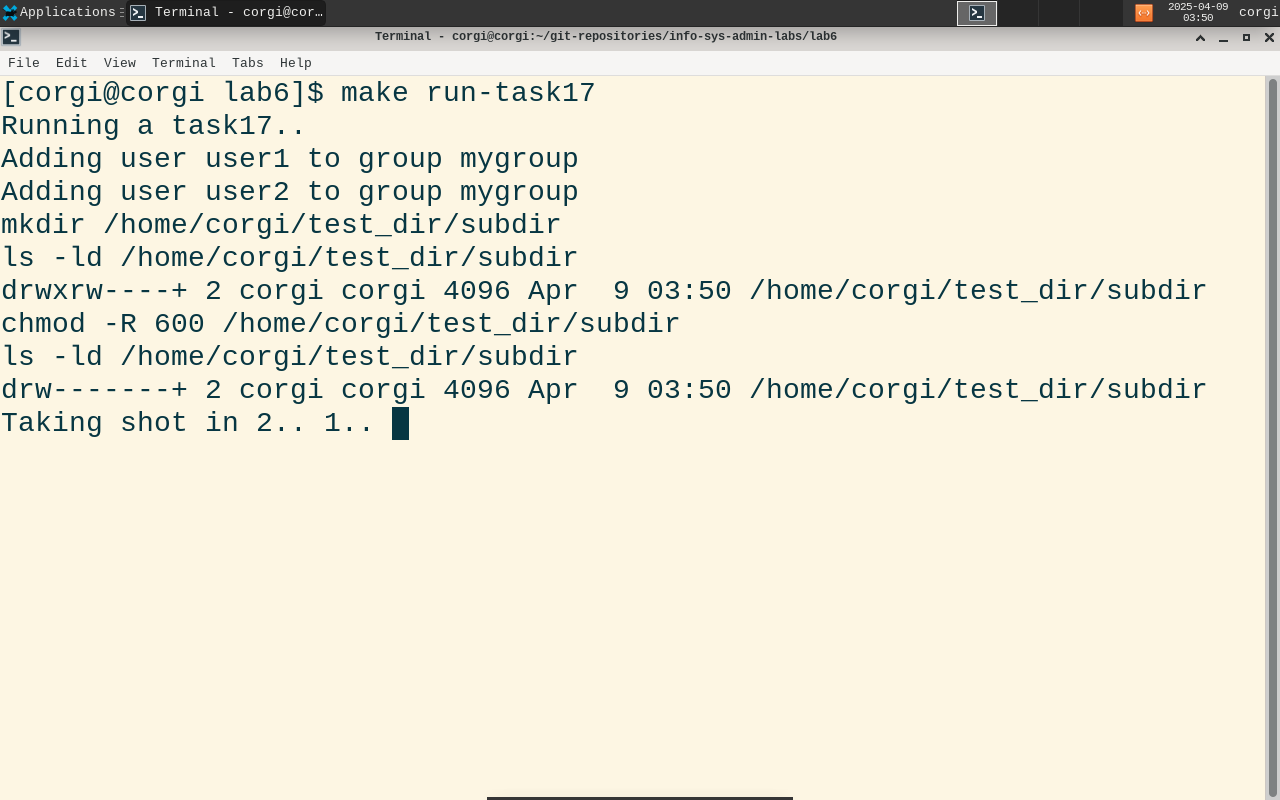
\includegraphics[width=500pt]{task17.png}
	\end{center}

	\subsection*{Задание 18}
	\addcontentsline{toc}{subsection}{Задание 18}
	Удалите пользователя \textit{user1} из системы.
	\lstset{style=mystyle}
	\lstinputlisting[language=Bash]{src/task18/main.sh}
	\begin{center}
		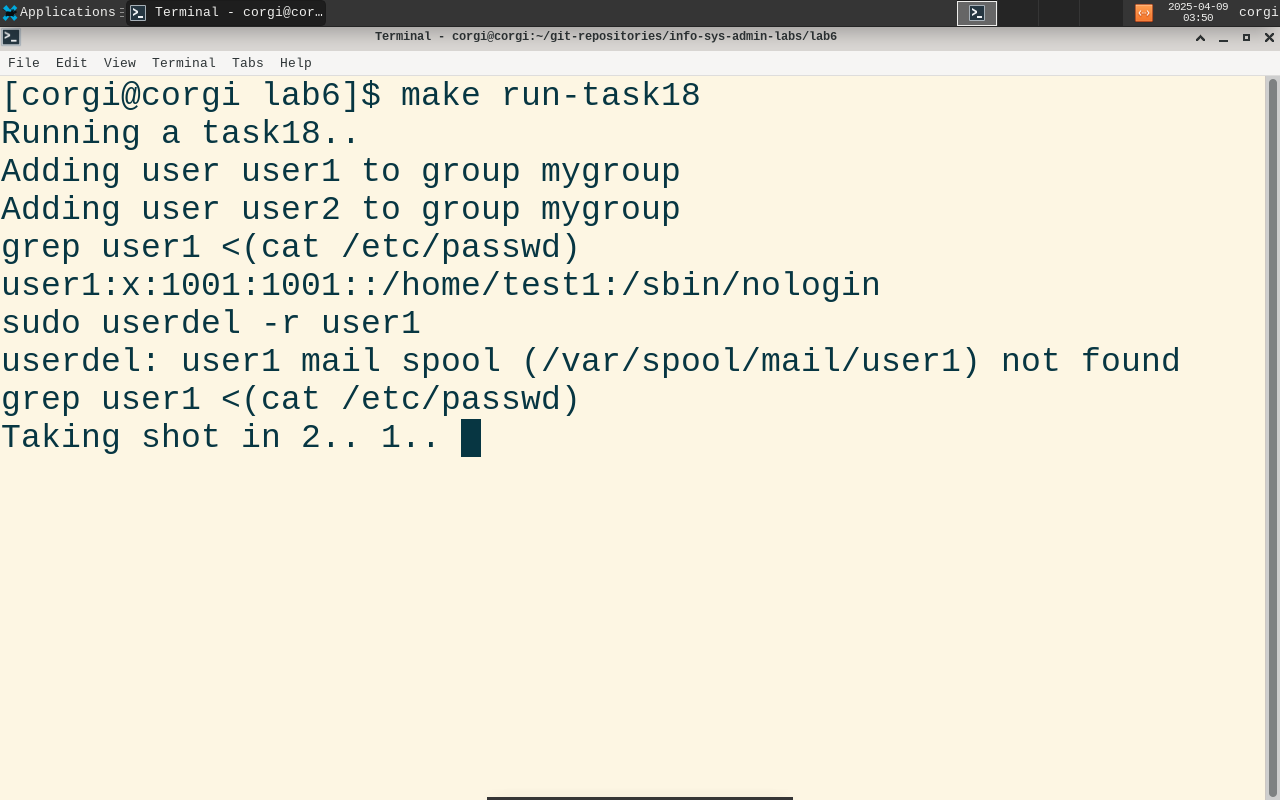
\includegraphics[width=500pt]{task18.png}
	\end{center}

	\subsection*{Задание 19}
	\addcontentsline{toc}{subsection}{Задание 19}
	Найдите в системе все файлы с установленными битами \underline{SUID} и посчитайте их количество. Проанализируйте список - для чего используются эти файлы?
	\lstset{style=mystyle}
	\lstinputlisting[language=Bash]{src/task19/main.sh}
	\begin{center}
		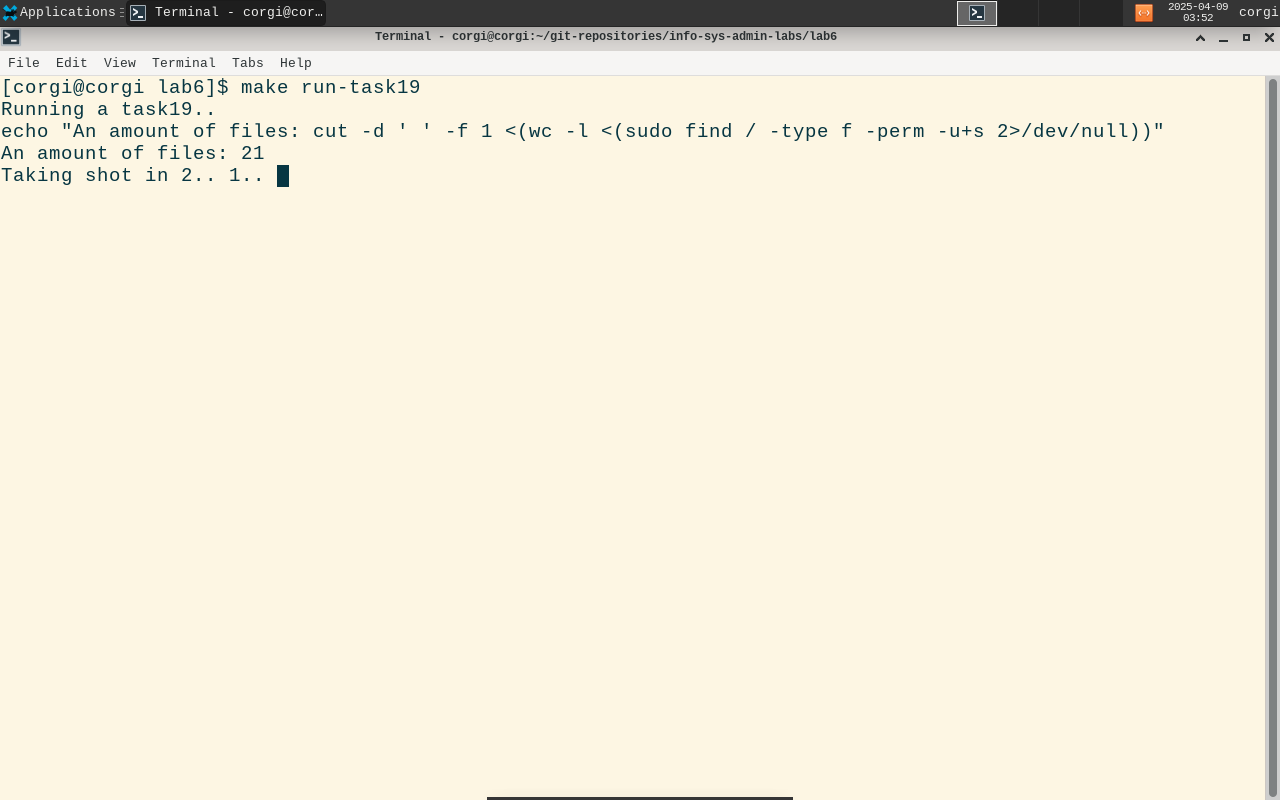
\includegraphics[width=500pt]{task19.png}
	\end{center}
\end{document}
